\documentclass{article}
\usepackage[utf8]{inputenc}
\usepackage[a4paper, total={5.5in, 9in}]{geometry}
\usepackage{biblatex}
\usepackage{todonotes}
\usepackage{amsmath}
\usepackage{titlesec}
\usepackage[T1]{fontenc}
\usepackage{nameref}

% Capitalize sections
\titleformat{\section}
  {\normalfont\fontsize{11pt}{12pt}\selectfont\bfseries}{\thesection}{1em}{\MakeUppercase}

\renewcommand\abstractname{ABSTRACT}
\renewenvironment{abstract}
 {\small
  \begin{center}
  \bfseries \abstractname\vspace{0em}
  \end{center}
  \list{}{
    \setlength{\leftmargin}{12.5mm}%
    \setlength{\rightmargin}{\leftmargin}%
  }
  \item\relax}
 {\endlist}

 \renewcommand{\arraystretch}{1.2}
 
\addbibresource{references.bib}

\title{\textbf{Norwegian Generative Chatbot using Personal Chat Log Data}}
\author{Torjus Iveland \and Vegar Andreas Bergum}
\date{}

\begin{document}

\maketitle
\centerline{\textit{TDT4310 - Intelligent Text Analytics and Language
Understanding}}
\centerline{\textit{Norwegian University of Science and Technology}}
\centerline{\textit{Trondheim, Norway --- April 2019}}
\vspace{6mm} % Space above abstract

\begin{abstract}

This report explores the state of Norwegian chatbot systems with
the aim of verifying that conventional English chatbot creation techniques
also can be used to create chatbots which converse in Norwegian. There are
multiple challenges with Norwegian chatbots, due to the syntactic structure
of the language as well as the lack of available training data.

\paragraph{}
We present an implementation of a generic-domain chatbot system using a simple
sequence-to-sequence model with attention, a kind of model which primarily is
applied to neural machine translation but which also has proven effective for
chatbot systems. We believe our results illustrate that neural machine
translation techniques indeed can be applied to create chatbots in both
Norwegian as well as English, as long as enough training data of a
sufficiently high quality is available. However, we stress that in many cases
such training data in Norwegian can be hard to obtain.  

\end{abstract}

\vspace{3mm}

\section*{Introduction}
A chatbot is a computer system which can interact with a user through natural
language. Because humans tend to prefer more human-like interfaces, chatbots
can be very useful in applications such as customer support, education, and
personal productivity systems like Google Assistant. This project concerns
such chatbots which converse specifically using the Norwegian language.

\paragraph{}
Most research on chatbot systems concerns chatbots which converse in English.
However, Norwegian has a syntactic structure which differs from that of
English. Therefore, it is not guaranteed that this research automatically
applies to Norwegian chatbots as well. Additionally, further problems arise
from the fact that training data in Norwegian is not as abundant as for
English.

\paragraph{}
In this project, we explore Norwegian chatbots, with the goal of verifying that
conventional chatbot-creation techniques also can function adequately in
Norwegian. We especially want to verify that deep learning techniques such as
sequence-to-sequence models \cite{Cho2014} can be used to create
general-purpose Norwegian chatbots. Such models are usually used for machine
translation, but they have also proven effective in the field of chatbots.
Therefore, the main objective of this project is to implement a simple Norwegian
chatbot using a sequence-to-sequence model with an attention mechanism
\cite{Bahdanau2015}, which for example could be used as a small talk module in
another mode domain-specific chatbot.

\paragraph{}
We differ between retrieval-based and generative chatbots. A retrieval-based
system usually maps user input to a predefined intent, and then retrieve an
answer from a set of answers belonging to the detected intent. A generative
system does not rely on such predefined sets of answers.  Instead, they are
able to automatically generate an answer to the provided query. In this
project, we restrict ourselves to the latter kind of model. We also restrict
ourselves to an user-initiative only model, which means that the chatbot simply
responds with an answer to each user query.

\if
- Something about how we want to structure the rest of the report.  
- Fix that goal, motivation, question and hypothesis are not clear.  
\fi

\section*{Method}
% I dette kapitlet skal du skrive om hvordan du har gått frem metodisk, og vise
% hvordan valg av design og metode egner seg til å svare på problemstillingen
% din.  Kapitlet må kunne gi svar på disse spørsmålene: Hvordan samlet du inn
% datamaterialet?  Hvordan behandlet du dataene du samlet inn?  Hvorfor valgte
% du disse metodene?  Hva er styrkene og svakehetene ved disse metodene?  Du
% skal også si noe om hvorfor du har gjort din undersøkelse på den måten du
% gjorde – og da peke på styrker og svakheter. I tillegg skal du drøfte etiske
% aspekter ved prosjektet. På den måten viser du at du har kommet frem til
% resultatene på en pålitelig og troverdig måte, men også at du er reflektert
% og kritisk overfor arbeidet du har gjort.  Husk også at du her, slik som i
% teorikapitlet, bare skal skrive om det metodiske som er relevant for din
% studie.
\if
 - Ressursbegrensning (datakraft og tid) har begrenset omfanget på evaluering
 av forskjellige modeller
\fi

The main goal of this project was to explore the possibility of generative
chatbots using Norwegian. In order to do this, we implement a simple generative
chatbot model. We then train this model using both Norwegian and English data
in order to compare the effectiveness of the model for Norwegian with that of
English. The method of choice in this project was a simple sequence-to-sequence
model, as proposed by Cho et al. in their paper \cite{Cho2014}, with an
attention mechanism \cite{Bahdanau2015}. In order to compare the Norwegian and
English models, we provide our own observations of the model performance as
well as user evaluations of the systems, where we have gotten a set of people
to compare the models with each other.

\paragraph{}
One of the prerequisites for a language generation system such as a chatbot is
data in the language being generated. The langauge generation process greatly
depends on the amount and qualtity of the available data. In this project, we
perform comparisons using similar data conditions for both English and Norwegian,
in order to establish the effectiveness of the \emph{model} for Norwegian. We
trained an English chatbot using a subset of a corpus commonly used for English
chatbots, in order to compare the effectiveness of the model between English
and Norwegian for similarly sizd datasets. A discussion of the data used in this
project follows in the next section.

\paragraph{}
Sequence-to-sequence models have proven to be an excellent baseline for
chatbot models \cite{Vinyals2015}. When considering a user-initiative only
model the task of a generative chatbot system can be reduced to mapping an
input utterance to a target utterance. This is analogous to how the same type
of model is applied for neural machine translation. Chatbot models with a
sufficiently large corpus for such example-based ``translation'' have been
shown to produce promising results \cite{Ezquerra2018}. Although these bots are
not able to apply any real logic to their answers, they are certainly able to
mimic natural human language.

\paragraph{}
With appropriate additions to encoder-decoder models such models are able to
produce comparable results to state of the art phrase-based systems for machine
translation, as shown by Bahdanau, Cho \& Bengio in their paper on the attention
mechanism \cite{Bahdanau2015}. It is likely that attention mechanisms also can
provide better results for chatbots.

\paragraph{}
The model in this project utilises Google's Machine Learning framework
TensorFlow as a backend with Keras as a high-level wrapper. The architecture
utilises Gated Recurrent Units (GRU) with a three-dimensional sequence
embedding. The architecture has been extended with Bahdanau Attention, allowing
for the decoder inputs to consider a \textit{context} vector instead of the
entire encoder output.
\todo{I propose the paragraph in the source code, because three dimensional
sequence embedding doesnt really mean much. Also, I think we should consider
moving this paragraph out of this section.}
%The model in this project is implementing using TensorFlow, a machine learning
%framework by Google, with Keras as a high-level wrapper. The architecture is 
%a sequence-to-sequence model which utilises Gated Recurrent Units. The model
%has also been extended with Bahdanau attention, allowing for the decoder inputs
%to consider a concext vector instead of the entire encoder output.

\paragraph{}
This architecture can be further developed using a word-level embedding system
such as \textit{Word2Vec} \cite{word2vec}, or by incorporating a system such
as BERT \cite{bert2018}.

\section*{Data}
Norwegian chatbot training data is not readily available, but relevant corpora
still exist.  For example, multiple spoken language corpora are available
through the CLARINO project \cite{clarino-about}. Examples of CLARINO
corpora which might prove useful for a chatbot project are the Big Brother
corpus \cite{clarino-bb} and NoTa-Oslo \cite{clarino-nota}, which both provide
spoken language annotations for the Norwegian language. However, both these
corpora have quite restrictive licenses and are only accessible online for
privacy reasons. Thus, the CLARINO corpora are not well suited for our chatbot
usage.

\paragraph{}
Another possible data source is to use exports of personal chatbot data from
various online platforms, For example, Facebook allows users to export their
private Messenger chat data. If all parties involved in a conversation consent,
such data can be used to train a chatbot. An average Facebook user will quite
easily be able to generate several tens of thousands of utterances over the
course of a few years. More avid users of the platform can have chat logs
containing several hundred thousands or even millions of messages. This project
combines the utterances of two Facebook users, ending in a corpus with more
than 110 000 utterance pairs. However, processing such a dataset has proven a
challenge. With a maximum sequence length $max\_seq\_length$ of $20$, a
vocabulary size $vocab\_s$ of $5000$ and $110 000$ utterances stored in a
32-bit float format, storing it requires

\begin{align*}
  max\_seq\_length &\times vocab\_s \times 110,000 \times 32 \\
  &= 20 \times 5000 \times 110,000 \times 32 = 3.5 \times 10^{10} \text{ bytes}\\
  &= 352 \text{ GB}
\end{align*}

of memory. During this project, only 32GB of memory was available at a
time, and so the usable corpus was reduced to 10 000 utterances, a tenth
of the original corpus size.

\paragraph{}
In addition to using personal Facebook Messenger data, the Cornell Movie
Dialogs Corpus \cite{cornell-corpus} has been used for model evaluation.
The Cornell corpus consists of several hundred thousands of utterances
from movie scripts that are freely available, and has proven effective
an effective baseline for training of English chatbots. We therefore use
a subset of this corpus in order to evaluate the effectiveness of our model
for English and Norwegian under similar conditions.

\section*{Implementation}
Chatbots which utilise deep learning are usually based on sequence to sequence
models. A sequence to sequence model is a type of architecture where there is
an encoder RNN and a decoder RNN. For usages such as machine translation and
chatbots, the idea is that we feed the encoder RNN input words one at a time,
which eventually results in an output vector describing the input sentence.
This output vector is sometimes referred to as a thought vector, as it stores
the system's understanding of the input. For machine translation, we would feed
the encoder RNN the sentence to be translated, and for chatbots, the encoder
RNN would accept the input sentence which should be responded to. The decoder
RNN is trained to take context vectors from the attention layer and output
tokens from the encoder one by one until an end of sequence token is outputted.
Since the decoder network is dependent on the output of the encoder network and
the attention mechanism, all three are trained together. This model has proven
very effective for neural machine translation and other tasks as well. An early
description of this architecture is available in \cite{Cho2014} and
\cite{Bahdanau2015}.
\todo{Maybe output vector -> final encoder state, instead of output = thought vector?
Check this paragrah out.}

\paragraph{}
The rest of this section is dedicated to describing the architecture of
this project. We first describe the preprocessing phase, then the model which
is being used, and finally the inference phase, in which the responses to user
utterances are actually generated.

\subsection*{Preprocessing}
Before the data is forwarded to the model, it needs to be preprocessed. The
preprocessing phase in this project consists of a number of steps. We use
data from Facebook Messenger to train our chatbot. To split the data into
input and target data sets, we simply treat each utterance as the input to
the next utterance - that is, each utterance is the response to the previous.

\paragraph{}
First, the text is normalized by removing all punctuation from the text. Newlines
are replaced with spaces, and all text is converted to lower-case. Ideally,
the bot should output grammatically correct text, but this requires a
significantly more complex model. We use the Norwegian NLTK tokenizer to split
the text into words. Lastly, each utterance is wrapped in a special start and
end token, which indicates to the model when it should stop generating text
during the inference phase.

\paragraph{}
The preprocessing system also performs filtering on which utterances should
and should not be used. For example, the system can be configured to only
use responses from a specific person, to give the chatbot a more distinct
personality. Additionally, the system can removes self-replies, so that
only discourse between two different persons is considered.

\paragraph{}
The maximum length of an input or target utterance is capped at 20 tokens.
This is required to reduce the size of the input matrices for the model, due
to limited available computational power. However, an analysis of the dataset
shows that only about 4\% of the utterances are above this limit. Similarly,
we limit the number of words which may appear in the input and target data.
This vocabulary size only includes the most common 3000 words. In accordance
with Zipf's law, 3000 words account for slightly under 80\% of the total
vocabulary. While this might reduce the quality of the output due to certain
parts of the output sentences being omitted, it is crucial that the size of
the input vectors are minimized.

\subsection*{Feature extraction}
The preprocessing system also provides a way of encoding utterances as
vectors, a process known as word embedding. This is done by simply
encoding each token as a unique number, with additional logic for handling
unknown tokens. Note that this is a very simple embedding technique, and
therefore future work might include exploring alternative embedding techniques
such as \emph{Word2Vec} \cite{word2vec} or \emph{BERT} \cite{bert2018}.
We now provide a high-level conceptual overview of the feature extraction
process used in this project.

\paragraph{}
With a corpus $D = \{\text{``How are you doing?''}\}$ containing utterances, 
a vocabulary $\vec{V}$ containing all distinct words in the corpus is
constructed. This is used to build a mapping where each token is mapped to
its corresponding index in the vocabulary vector $\vec{V}$. This mapping is
then used to encode utterances as vectors. Table 1 illustrates
%WATCHOUTWATCHOUTWATCHOUTWATCHOUTWATCHOUTWATCHOUTWATCHOUT
this mapping. Note that there are three special tokens representing the
beginning of the sequence, padding and end of the sequence.

$$
   \vec{V} = [ \textrm{<BOS>},\, \textrm{<PAD>},\, \textrm{``how''},\,
               \textrm{``are''},\, \textrm{``you''},\, \textrm{``doing''},\,
               \textrm{<EOS>}]
$$

\begin{table}[hbt]
  \begin{center}
    \begin{tabular}{c|c|c|c|c|c|c|c}
      \textbf{Index} & 0 & 1 & 2 & 3 & 4 & 5 & 6 \\
      \hline
      \textbf{Token} & <PAD> & <BOS> & how & are & you & doing & <EOS> \\
    \end{tabular}
  \end{center}
  \label{tab:tok2num}
  \caption{Token to number mapping}
\end{table}

\paragraph{}
In order to maintain a fixed dimensionality of our sequence embeddings, there
needs to be predefined sequence length. In this example, this is set to 5. If a
sequence is shorter than this, the rest of the sequence matrix is filled with
padding tokens. Using the vocabulary above, the word ``how'' is mapped to the
word vector $\vec{v}_2$.

$$
  \vec{v}_2 = [0, 0, 1, 0, 0, 0, 0] \quad {\leftrightarrow} \quad \textrm{``how''}
$$

\paragraph{}
Using these word vectors, a matrix of one-hot encoded row vectors can be
constructed. This matrix $d_0$ is the embedding of the utterance sequence
in the initial dataset $D$.  

$$
  d_{0} = 
    \begin{bmatrix}
      0 & 1 & 0 & 0 & 0 & 0 & 0\\
      0 & 0 & 1 & 0 & 0 & 0 & 0\\
      0 & 0 & 0 & 1 & 0 & 0 & 0\\
      0 & 0 & 0 & 0 & 1 & 0 & 0\\
      0 & 0 & 0 & 0 & 0 & 1 & 0\\
      1 & 0 & 0 & 0 & 0 & 0 & 0\\
      0 & 0 & 0 & 0 & 0 & 0 & 1\\
    \end{bmatrix}
$$

\paragraph{}
Equation \ref{eq:seq-out} show the exact sequence represented by $d_0$. Notice
that its length is 5, excluding the beginning- and end of sequence tokens.

\begin{equation} \label{eq:seq-out}
  [ \textrm{<BOS>},\, \textrm{``How''},\, \textrm{``are''},\, \textrm{``you''},\,
    \textrm{``doing''},\, \textrm{<PAD>},\, \textrm{<EOS>} ]
\end{equation}

\paragraph{}
This sequence embedding is used to extract the necessary features needed to
make a statistical prediction of the next token in an output sequence, given an
input sequence. The extracted features are the context of the token's
occurrences.

\subsection*{Model}
This project utilises a fairly standard sequence-to-sequence model with
attention implemented using Keras, which is illustrated in figure
\ref{fig:keras-model}. Keras and TensorFlow does not natively support
attention resulting in using a custom implementation of an attention layer
\cite{keras-attention} that has been heavily modified to fit into the rest of
the Keras model.  

\paragraph{}
The encoder consists of an input layer with dropout and a GRU
layer which feeds its hidden states into the decoder GRU and its outputs into 
the attention layer. The decoder consists of an input layer with dropout that
feeds the decoder GRU alongside the encoder GRU hidden state. The decoder GRU
outputs is also fed into the attention layer. The attention layer takes in, as
mentioned, the encoder and decoder outputs. The decoder outputs and the
attention outputs are then concatenated and fed into the activation function of
the decoder, which actually makes a prediction.

\paragraph{}
In this model, the encoder GRU is fed one-hot encoded utterances one at a
time. Recall that the purpose of this step is to create a compact, internal
representation of the input utterance - a thought vector, so to speak. The
encoder GRU outputs a list containing outputs from the encoder as well as the
internal encoder state. The decoder GRU discards the GRU output but uses the
final hidden encoder state as its own initial state, so that the decoder also
has information about the input utterance. As input, the decoder activation
layer is fed a concatenation of the decoder GRU outputs and the attention layer
outputs. Note that the attention layer output is a function of the encoder
outputs and the decoder GRU outputs.
\todo{For these two paragraphs, check state vs output?}

\begin{center}
  \begin{figure}[hbt]
    \centering
    \makebox[\linewidth][c]
      {
        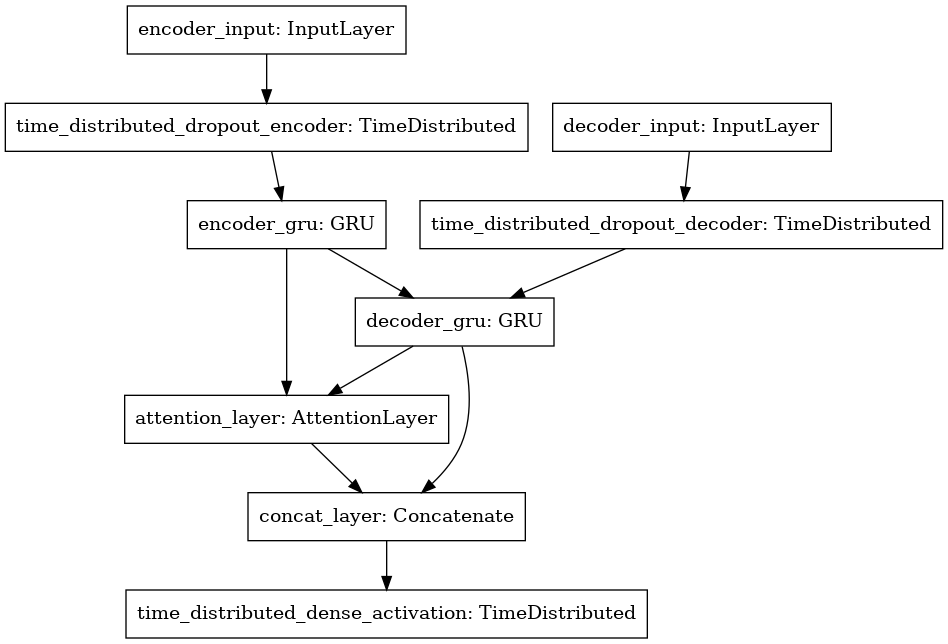
\includegraphics[width=1.1\textwidth]
        {model.png}
      }
    \caption{The Keras model behind the chatbot.}
    \label{fig:keras-model}
  \end{figure}
\end{center}

During training the decoder is fed the target sequence - that is, the target
utterance. As a target for the output, the decoder is fed the same target utterance, shifted to the right by one.
This is a training method which is known as teacher forcing
\cite{teacher-forcing}. It simply means that the network is taught to output
token $n$ in the utterance, given token $n-1$ as input. The alternative to
teacher forcing is to feed the decoder prediction back into the decoder output,
instead of always using the ground truth as the decoder input. However, not
using teacher forcing generally makes training slower and the model unstable.

For training, we use the built-in Keras training functionality. We use the
\emph{rmsprop} optimizer and \emph{categorical crossentropy} as the loss
function. All models were trained for between 200 and 300 epochs, depending
on the size of the dataset. We used a batch size of 64.

\subsection*{Inference}

Once a model is trained, we can use it to generate responses to input
utterances. This is a separate phase from the training phase, which is usually
referred to as the inference phrase. We now provide a high-level description
of the inference phase used in this chatbot system.

\paragraph{}
When the system receives an input utterance from the user, we first run the
preprocessing step on the utterance to ensure it conforms to the same
specifications as the input data used while training. Then, this processed
input utterance is fed to the encoder, and the final hidden encoder state is
used as the initial state for the decoder, just as in the training phase.
Recall that only the decoder GRU uses the hidden encoder state. The dense
activation layer of the GRU that actually makes the prediction, uses the
context state given by the attention layer. We then run the decoder, using the
special \emph{<BOS>} token as the input. This yields the initial token of the
response utterance. The system then feeds this token back into the decoder and
uses it to generate the next token in the utterance. At each step in this
process, the system picks the most likely token. This process halts when the
special \emph{<EOS>} token is generated, at which point the response utterance
is returned to the user.

\paragraph{}
The inference system just described is a greedy decoding scheme, as the token
picked is always just the most likely token. However, this basic scheme does
not always yield the most likely \emph{utterance}. Future work might explore
alternative inference schemes based on algorithms such as beam search, which
seek to maximize the probability for the entire output utterance.

% Architecture \ Experimental Setup + Teacher forcing Future work: Bert/custom
% embeddings, embedding layer, bidirectional model, beam search

\section*{Related Work}
Multiple Norwegian chatbots already exist. However, these are usually systems
which first map the user query to a predefined intent, and then retrieve an
answer from a list of answers belonging to the intent. Such systems require a
fair amount of manual training and lack the ability to independently formulate
an answer independently, based only on the question.  In this report, we
describe a generative chatbot which is based on an unsupervised model.
\todo{Elaborate more in this section.}

\section*{Results}
% Å analysere gjør du ved å redegjøre, forklare og vurdere funnene dine.
% Analysedelen av oppgaven blir ofte kalt resultater, slik som i
% IMRoD-modellen.  I kvantitative studier vil du kanskje i tillegg til å
% presentere funnene skriflig, bruke figurer og tabeller for å gi leseren en
% oversikt og innsikt i hva du har gjort.  I empirisk baserte studier vil
% analysene handle om å beskrive og tolke. Mange vil ofte drøfte enkeltfunnene
% i dette kapitlet og ta for seg mer overordnede funn i drøftingskapitlet.

The training phase of a chatbot is difficult. The calculated loss during
training is not a good metric since there is no good objective measure of how
good a response is. Although, after 300 epochs of training on datasets of
10,000 utterances the model converged at a loss of ~0.1, using the
\textit{categorical crossentropy} function.

\paragraph{}
Once the model was fully trained, supervised human evaluation would be used to
establish a score. This was done by attempting to converse with the chatbot. 
This project is concerned with Norwegian chatbots. In order to establish a
baseline for comparison the same model was trained with the same amount of data
from the Cornell Movie Dialog dataset \cite{cornell-corpus}. The results of the
conversations are found in table 2 and 3 for the Norwegian and English versions
respectively.

\begin{table}[hbt!]
\centering
\begin{minipage}{.5\linewidth}
  \begin{tabular}{rp{5cm}}
    \textbf{Human:} & hei\\
    \textbf{Bot:} & går det greit\\
    \textbf{Human:} & ja det går fint\\
    \textbf{Bot:} & nei\\
    \textbf{Human:} & jeg sa akkurat at jeg har det fint\\
    \textbf{Bot:} & har ikke noen den så mye men du ikke å\\
    \textbf{Human:} & er du levende\\
    \textbf{Bot:} & ok\\
    \textbf{Human:} & er det et ja\\
    \textbf{Bot:} & e e det\\
    \textbf{Human:} & du skremmer meg \\
    \textbf{Bot:} & nei\\
    \textbf{Human:} & jo, jeg blir skremt\\
    \textbf{Bot:} & så det er jo smud\\
  \end{tabular}
\end{minipage}%
\begin{minipage}{.5\linewidth}
  \begin{tabular}{rp{10cm}}
    \textbf{Human:} & er du på gløs?\\
    \textbf{Bot:} & ja\\
    \textbf{Human:} & har du bord?\\
    \textbf{Bot:} & ja\\
    \textbf{Human:} & nice\\
    \textbf{Bot:} & nei det er ikke noe særlig\\
    \textbf{Human:} & er det pk på kontoret?\\
    \textbf{Bot:} & kanskje\\
    \textbf{Human:} & kan du sjekke for meg\\
    \textbf{Bot:} & nei\\
    \textbf{Human:} & da får jeg ha med selv\\
    \textbf{Bot:} & hmm\\
    \textbf{Human:} & hmm\\
    \textbf{Bot:} & for et liv\\
  \end{tabular}
\end{minipage}%
\caption{Norwegian logs}
\end{table}

\begin{table}[hbt!]
\centering
\begin{minipage}{.5\linewidth}
  \begin{tabular}{rp{5cm}}
    \textbf{Human:} & hi\\
    \textbf{Bot:} & hey there tired of\\
    \textbf{Human:} & are you tired of me?\\
    \textbf{Bot:} & let me see a long\\
    \textbf{Human:} & a long what?\\
    \textbf{Bot:} & how much\\
    \textbf{Human:} & what do you want\\
    \textbf{Bot:} & in the sight of god that is a sin\\
    \textbf{Human:} & please forgive me\\
    \textbf{Bot:} & im no i was to been to you for did its\\
    \textbf{Human:} & you make no sense now\\
    \textbf{Bot:} & thats not you there to the\\
    \textbf{Human:} & alright\\
    \textbf{Bot:} & alright\\
  \end{tabular}
\end{minipage}%
\begin{minipage}{.5\linewidth}
  \begin{tabular}{rp{10cm}}
    \textbf{Human:} & are you on campus?\\
    \textbf{Bot:} & well i have to be there to that\\
    \textbf{Human:} & what are you doing there\\
    \textbf{Bot:} & there\\
    \textbf{Human:} & right\\
    \textbf{Bot:} & oh yeah\\
    \textbf{Human:} & wanna go eat lunch\\
    \textbf{Bot:} & what\\
    \textbf{Human:} & a baguette\\
    \textbf{Bot:} & whats that\\
    \textbf{Human:} & it is a food\\
    \textbf{Bot:} & take a round all do you\\
    \textbf{Human:} & it is a french food\\
    \textbf{Bot:} & he has a little\\
  \end{tabular}
\end{minipage}%
\caption{English logs}
\end{table}

\paragraph{}
From the logs it is clear that the chatbot is able to respond in a natural way
to some utterances. The conversation is not necessarily coherent due to the
lack of context, but rather a single focus on the last utterance. The bot is
able to construct some valid sentences, but the lack of a defined grammar or
rules makes it subject to sentence generation that is invalid.
From the limited conversational data it becomes clear that the Norwegian
version is comparable to the English version, if not slightly better.

\section*{Discussion / Evaluation}
% Du skal her drøfte resultatene dine og sette dem inn i en sammenheng. Å
% drøfte vil si å: sette ulike synspunkter, momenter, argumenter, faktorer og
% årsaker opp mot hverandre vurdere og sette dem opp mot hadily available, this
% is one of the primary challenges.  + Facebook Messenger data dump.  +
% Clarino: Tried, but restrictive licenses.  + Movie scripts. Copyright
% unclear.

% heavily biased dataset bad training data, not so much training data simple
% model

% heavily biased dataset
% bad training data, not so much training data
% simple model

In order to get a better view of the performance of the model, a few human
evaluators were given access to each version of the chatbot. The evaluators
were told that they are conversing with a small-talk chatbot, and were given
instructions to talk to them. Once they had conversed the with bots for a few
minutes, they were asked to rank the bots on a scale from 0 to 10, where 0
is equivalent to having a monologue while 10 is the equivalent to conversing
with a human being. The resulting scores are found in table 4.

\begin{table}[hbt!]
    \centering
    \begin{tabular}{|c|c|}
        \hline
        \textbf{Norwegian} & \textbf{English}\\
        \hline
        3 & 1\\
        4 & 3\\
        5 & 2\\
        1 & 1\\
        3 & 2\\
        2 & 6\\
        \hline
        \textbf{Avg: 3} & \textbf{Avg: 2.5}\\
        \hline
    \end{tabular}
    \caption{Evaluation results}
    \label{tab:evaluation-results}
\end{table}

\paragraph{}
From the scores we can see that there is a slight preference for the Norwegian
chatbot, which correlates well with the resulting logs discussed earlier.
However, the scores are relatively low, which might be due to high expecations
from the evaluators. The evaluators were often attempting to converse within
a large range of topics which will yield poorer results when considering the
relatively small dataset used (10,000 samples).

\section*{Conclusion}
% Om avslutningen din skal være en konklusjon eller en oppsummering, avhenger
% av problemstillingen din. En konklusjon skal svare på problemstillingen, mens
% en oppsummering gjentar det viktigste fra oppgaven. Det er ikke uvanlig å
% velge en kombinasjon av de to, hvor du både oppsummerer oppgaven kort, men
% også svarer på problemstillingen.  Det er lurt å la avslutningen speile
% innledningen, ved å si hva du har gjort. Avslutningen bør også sette oppgaven
% din i et større perspektiv, og peke på hvilke muligheter du ser ut fra ditt
% prosjekt. Hvilke bidrag har din undersøke gitt til faget? Er det noe som
% burde blitt studert ytterligere? Slik tar du utgangspunkt i ditt eget
% prosjekt og peker på mulighet for oppfølging.

\todo{Conversation data in appendix.}

\printbibliography

\end{document}
